\documentclass[a4paper, 11pt, notitlepage]{article}

%\usepackage{babel}
\usepackage[utf8]{inputenc}
\usepackage[T1]{fontenc, url}
\usepackage{textcomp}
\usepackage{amsmath, amssymb}
\usepackage{amsbsy, amsfonts}
\usepackage{graphicx, color}
\usepackage{parskip}
\usepackage{framed}
\usepackage{amsmath}
\usepackage{xcolor}
\usepackage{multicol}
\usepackage{url}
\usepackage{flafter}
\usepackage{caption}

%\DeclareCaptionLabelSeparator{colon}{. }
\renewcommand{\captionfont}{\sffamily}
\renewcommand{\captionlabelfont}{\bf\sffamily}
\setlength{\captionmargin}{40pt}

\usepackage{geometry}
\geometry{headheight=0.01mm}
\geometry{top=24mm, bottom=29mm, left=39mm, right=39mm}

\renewcommand{\arraystretch}{2}
\setlength{\tabcolsep}{10pt}
\makeatletter
\renewcommand*\env@matrix[1][*\c@MaxMatrixCols c]{%
  \hskip -\arraycolsep
  \let\@ifnextchar\new@ifnextchar
  \array{#1}}
%
% Parametere for inkludering av kode fra fil
%
\usepackage{listings}

\DeclareMathAlphabet{\mathbfit}{OML}{cmm}{b}{it}

\definecolor{javared}{rgb}{0.6,0,0} % for strings
\definecolor{javagreen}{rgb}{0.25,0.5,0.35} % comments
\definecolor{javapurple}{rgb}{0.5,0,0.35} % keywords
\definecolor{javadocblue}{rgb}{0.25,0.35,0.75} % javadoc

\lstset{language=python,
basicstyle=\ttfamily\scriptsize,
keywordstyle=\color{javapurple},%\bfseries,
stringstyle=\color{javared},
commentstyle=\color{javagreen},
morecomment=[s][\color{javadocblue}]{/**}{*/},
% numbers=left,
% numberstyle=\tiny\color{black},
stepnumber=2,
numbersep=10pt,
tabsize=4,
showspaces=false,
captionpos=b,
showstringspaces=false,
frame= single,
breaklines=true}
%
% Definering av egne kommandoer og miljøer
%
\newcommand{\dd}[1]{\ \text{d}#1}
\newcommand{\f}[2]{\frac{#1}{#2}} 
\newcommand{\beq}{\begin{equation}}
\newcommand{\eeq}{\end{equation}}
\newcommand{\bra}[1]{\langle #1|}
\newcommand{\ket}[1]{|#1 \rangle}
\newcommand{\braket}[2]{\langle #1 | #2 \rangle}
\newcommand{\braup}[1]{\langle #1 \left|\uparrow\rangle\right.}
\newcommand{\bradown}[1]{\langle #1 \left|\downarrow\rangle\right.}
\newcommand{\av}[1]{\left| #1 \right|}
\newcommand{\op}[1]{\hat{#1}}
\newcommand{\braopket}[3]{\langle #1 | {#2} | #3 \rangle}
\newcommand{\ketbra}[2]{\ket{#1}\bra{#2}}
\newcommand{\pp}[1]{\frac{\partial}{\partial #1}}
\newcommand{\ppn}[1]{\frac{\partial^2}{\partial #1^2}}
\newcommand{\up}{\left|\uparrow\rangle\right.}
\newcommand{\upup}{\left|\uparrow\uparrow\rangle\right.}
\newcommand{\down}{\left|\downarrow\rangle\right.}
\newcommand{\downdown}{\left|\downarrow\downarrow\rangle\right.}
\newcommand{\updown}{\left|\uparrow\downarrow\rangle\right.}
\newcommand{\downup}{\left|\downarrow\uparrow\rangle\right.}
\newcommand{\bupup}{\left.\langle\uparrow\uparrow\right|}
\newcommand{\bdowndown}{\left.\langle\downarrow\downarrow\right|}
\newcommand{\bupdown}{\left.\langle\uparrow\downarrow\right|}
\newcommand{\bdownup}{\left.\langle\downarrow\uparrow\right|}
\renewcommand{\d}{{\rm d}}
\newcommand{\Res}[2]{{\rm Res}(#1;#2)}
\newcommand{\To}{\quad\Rightarrow\quad}
\newcommand{\eps}{\epsilon}
\newcommand{\inner}[2]{\langle #1 , #2 \rangle}


\newcommand{\bt}[1]{\boldsymbol{#1}}
\newcommand{\mat}[1]{\textsf{\textbf{#1}}}
\newcommand{\I}{\boldsymbol{\mathcal{I}}}
\newcommand{\p}{\partial}
%
% Navn og tittel
%
\author{Jonas van den Brink \\[-0.2cm] \texttt{j.v.d.brink@fys.uio.no}}
\title{Introduksjon til programmering \\ Bjørnegård Skole}


\begin{document}


% \maketitle

\thispagestyle{empty}
\vspace{1.8cm}


\begin{equation}
\frac{\d f}{\d x} = \lim_{\Delta x \to 0} \frac{f(x+\Delta x) - f(x)}{\Delta x}
\end{equation}

This definition supposes that the change $\Delta x$ becomes infinitesimal. 

Instead, we can choose $\Delta x$ to be a small constant, in that case we can approximate the derivative of the function by
\begin{equation}
\frac{\d f}{\d x} \approx \frac{f(x+\Delta x) - f(x)}{\Delta x} \quad \Delta x \ll 1
\end{equation}

$$f'(x) \approx \frac{f(x+\Delta x) - f(x)}{\Delta x}$$

$$f'(x_i) \approx \frac{f(x_{i+1}) - f(x_i)}{\Delta x}.$$

$$f(x_{i+1}) \approx f(x_i) + f'(x_i)\Delta x.$$

\section{Example}

$$u' = -u.$$

Known analytical solution
\begin{align*}
\frac{\d u}{\d x} = -u, \\
\frac{1}{u} \du = -\d x, \\
\ln u = -x + c, \\
u(x) = Ce^{-x}.
\end{align*}

Can calculate this as
$$u_{i+1} = (1-\Delta x) u_i, \quad \forall x=1,2,3,4,5,\ldots.$$
We of course have to know $u_0$

So we have
\begin{lstlisting}
x_0 = 0
x_1 = 2
N = 1001 # N should be big, so that dx becomes small

x = linspace(x_0, x_1, N) # H
dx = x[1]-x[0]

for i in range(N):
	u[i+1] = (1-dx)*u[i]

plot(x, u)
show()
\end{lstlisting}

This method is known as Euler's method

% \section*{Oppgave 1}
% \begin{itemize}
%     \item[(a)] Lag et skript som skriver ut teksten "Hello, World!" til skjermen.
%     \item[(b)] Lag et skript som skriver ut verdien av 4*5+2 til skjermen, blir resultatet annerledes om du skriver 2+4*5?
%     \item[(c)] Lag et skript som regner ut $2^{10}$ og skriver resultatet til skjermen.
%     \item[(d)] Lag et skript som regner ut $\sqrt{3}$ og skriver resultatet til skjermen. Her må du først importere \verb+sqrt+-kommandoen (squareroot) fra pylab.
% \end{itemize}

% \section*{Oppgave 2}
% For å regne oss om fra en temperatur oppgitt i grader Celsius $C$, til grader oppgitt i Fahrenheit $F$, bruker vi formelen
% $$F = \frac{9}{5}C + 32.$$
% \begin{itemize}
%     \item[(a)] Lag et skript som regner ut temperaturen i Fahrenheit for en gitt temperatur i Celsius.
%     \item[(b)] Bruk skriptet til å finne ut hvor mange grader Fahrenheit disse tempraturene er: $20^\circ$, $0^\circ$, $-40^\circ$.
% \end{itemize}

% \section*{Oppgave 3}
% \begin{itemize}
%     \item[(a)] Skriv et skript der du lagrer et fornavn og et etternavn. Skriv ut en beskjed til personen.
%     \item[(b)] Skriv også ut antall tegn i fornavnet og etternavnet. For å gjøre dette skal du bruke kommandoen \verb+len(name)+ som gir lengden av en tekststreng, det vil si, antall karakter. For eksempel gir \verb+len("Jonas")+, resultatet 5.
% \end{itemize}


% \clearpage

% \section*{Videre lesing og oppgaveløsning}

% Hvis du har kommet deg så langt som dette, bra jobba! Jeg kommer til å utivde dette skrivet etterhvert som kurset går, så hvis du sjekker tilbake om en uke eller to er det nok en del mer info og fler oppgaver her. Men hvis du ikke klarer å vente på det, så skal jeg komme med et par kilder du kan bruke for å lære mer med en gang.

% \subsection*{Nettkurs fra Code Academy}

% Først så har vi Code Academy, en nettside som gir gratis nettkurs i mange forskjellige programmeringsspråk. Code Academy er helt genialt fordi de underviser programmering hands on, som vil si at du lærer ved å kode fra første sekund. Her er en link til begynnerkurset dems in Python

% \url{http://www.codecademy.com/tracks/python}


% \subsection*{Programmeringsnøtter fra Project Euler}

% Hvis du er ute etter en utfordring, så kan jeg anbefale Project Euler. Dette er en nettside som legger ut mattenøtter med en vri, vrien er at problemene skal løses med programmering. Ta en titt på oppgavene her, de stiger raskt i vansklighetsgrad, så start på de første!

% \url{https://projecteuler.net/problems}



% \

% Denne teksten er ment som en kort oppsummering av det vi håper å ha kommet igjen etter første uke. Programmering er en ferdighet det tar tid å lære seg, og den beste måten å lære det på er rett og slett å prøve seg frem. Vi håper derfor at dere tar dere tid til å se litt på programmering på egenhånd, og skriver noen korte, enkle, og kanskje teite programmer.

% \section*{Installasjon}

% Vi kommer til å bruke programmeringsspråket \emph{Python}. Det er i prinsippet gratis, og det finnes mange forskjellige versjoner, og mange forskjellige tillegspakker. Den enkleste måten å installere alt vi trenger for dette prosjektet er å installere en samlepakke som heter \emph{Enthought Canopy}. Den laster du ned fra linken her

% \hspace{2cm}\url{https://www.enthought.com/downloads/}.

% Når filen er ferdig lastet ned, kjører du den og følger instruksene. Du kan la alt av innstillinger stå på standard om du ikke har andre preferanser.

% Når du har installert Canopy, kan du starte programmet. Siden det er en samle\-pakke er det en del funksjonalitet vi ikke kommer til å bruke, så ikke bli skremt av det kanskje ser litt komplisert ut.

% \section*{Hva er egentlig programmering?}

% Programmering går ut på å gi instrukser til datamaskinen. Disse instruksene skriver vi inn som kommandoer i en tekstfil. Denne tekstfilen kan så \emph{kjøres} av datamaskinen, som da tolker kommandoene vi har skrevet. Det er det som er et dataprogram. Kommandoene vi skriver må følge et bestemt programmeringsspråk, og det finnes fryktelig mange slike språk idag. Vi kommer til å holde oss til Python, et av de mest brukte programmeringsspråkene idag. Python er også et fint språk å begynne med om man aldri har programmert før.

% Moderne datamaskiner er fryktelig raske, men de er desverre ikke særlig smarte. Når vi programmerer må vi derfor være flinke til å gi helt riktige instrukser, om vi gir feil instrukser vil enten datamaskinen ikke skjønne hva vi mener, eller den vil rett og slett gjøre feil ting. Du må ikke være redd for å gjøre feil når du programmerer, det greier man rett og slett ikke å unngå. Det viktige er at du prøver å forstå \emph{hva} som gikk galt, og hvordan man kan rette det opp. Selv de beste programmererene i verden bruker mye av tiden sin på å rette opp i feil i programmer. Feil i koden blir ofte kalt \emph{bugs}, og det å rette opp i dem blir derfor kalt \emph{bugfixing}.

% \section*{Vi setter igang}

% Om vi starter Canopy, og velger \emph{Editor}, får vi opp et vindu der vi kan skrive et slikt dataprogram. Du skriver da koden inn i det største vinduet øverst. Du kan lagre programmet ditt med det navnet du vil, men du må legge på endelsen \verb+.py+, for Python. Etter du har lagret programmet ditt, kan du kjøre det ved å klikke på \emph{Run}-knappen, som er en grønn pil på toppen av editoren. En snarvei for Run er \verb!ctrl+R!.

% La oss se på et eksempel på et enkelt dataprogram:
% \begin{lstlisting}
% # Calculating the area and volume of a football

% from pylab import pi 

% r = 10

% area = 4*pi*r**2
% volume = (4./3)*pi*r**3

% print "A football with radius:", r
% print "Has an area of:", area 
% print "And volume of:", volume
% \end{lstlisting}

% Her er det ikke viktig at du skjønner alt som skjer i detalj, men la oss prøve å skjønne hovedtrekkene. Når vi trykker på Run-knappen, starter programmet med å tolke det som er skrevet, linje for linje. La oss derfor forklare det som skjer nedover i programmet, linje for linje.

% \vspace{0.4cm}
% \begin{lstlisting}
% # Calculating the area and volume of a football
% \end{lstlisting}
% \vspace{-0.3cm}
% Fordi den første linjen begynner med tegnet \verb+#+, betyr det at denne linjen ikke tolkes av datamaskinen i det heletatt. Vi kaller en slik linje for en kommentar, og det er rett og slett en forklaringstekst til enten oss selv, eller andre som skal lese koden vår. Vi skjønner altså at dette enkle programmet skal regne ut arealet og volumet av en fotball. Merk også at hele linjen er en annen farge fra resten av koden, dette gjør Canopy for at det skal være lettere å tolke koden.

% \vspace{0.4cm}
% \begin{lstlisting}
% from pylab import pi
% \end{lstlisting}
% \vspace{-0.3cm}
% Denne linjen ser kanskje litt avansert ut, men her importeres rett og slett tallet $\pi$. Vi trenger $\pi$ for å regne ut arealet og volumet til en kule, men den er ikke originalt tilstede i Python, vi må \emph{importere} den fra tillegspakken \emph{pylab}. Det finnes veldig mange slike tileggspakker i Python, til mange forskjellige bruksomeråder. I vårt tilfelle inneholder Pylab alt vi kommer til å trenge.

% \vspace{0.4cm}
% \begin{lstlisting}
% r = 10
% \end{lstlisting}
% \vspace{-0.3cm}
% Her defineres det at det finnes en \emph{variabel} som heter $r$, og at den skal være 10. Utifra kommentaren på starten av programmet skjønner vi at dette mest sannsynligvis er radiusen til fotballen. Denne linjen sier altså at radiusen er 10.

% \vspace{0.4cm}
% \begin{lstlisting}
% area = 4*pi*r**2
% \end{lstlisting}
% \vspace{-0.3cm}
% Her regnes arealet til fotballen ut fra den matematiske formelen $4\pi r^2,$
% og resultatet lagres i en \emph{variabel} som kalles \verb+area+.

% \vspace{0.4cm}
% \begin{lstlisting}
% volume = (4./3)*pi*r**3
% \end{lstlisting}
% \vspace{-0.3cm}
% Og her regnes volumet ut fra $\frac{4}{3}\pi r^3$, og resultatet lagres i \verb+volume+.

% \vspace{0.4cm}
% \begin{lstlisting}
% print "A football with radius:", r
% print "Has an area of:", area 
% print "And volume of:", volume
% \end{lstlisting}
% \vspace{-0.3cm}
% Til slutt kommer tre veldig like linjer. Alle bruker kommandoen \verb+print+, som forteller Python at vi skal skrive et resultat til skjermen, slik at brukeren kan lese det. Tekst vi skriver omsluttes av fnutter: \verb+"+, og vi ber Python skrive ut resultatene av utregningene etter teksten.

% Når programmet kjøres, får vi dette resultatet:
% \begin{lstlisting}
% A football with radius: 10
% Has an area of: 1256.63706144
% And volume of: 4188.79020479
% \end{lstlisting}

% \section*{Variabler og regning}
% I eksempelet vi nettopp så på, ble vi introdusert til et veldig viktig konsept i programmering, nemlig variabler. Variabler bruker vi når vi vil at datamaskinen skal huske på en verdi vi gir den, eller noe den regner ut.

% Hvis vi for eksempel skriver
% \begin{lstlisting}
% a = 6
% \end{lstlisting}
% \vspace{-0.3cm}
% vil datamaskinen opprette en variabel som heter \verb+a+, som inneholder \emph{verdien} 1. Den vil så huske på denne variabelen helt til programmet er ferdig å kjøre. Hvis vi for eksempel vil skrive ut innholdet av en variabel til skjerm, bruker vi \verb+print+ commandoen, så å skrive
% \begin{lstlisting}
% print a
% \end{lstlisting}
% \vspace{-0.3cm}
% gjør at det skrives ut et ettall til skjermen.

% Vi kan også regne med en eller flere variabler. Hvis vi for eksempel også definerer en variabel \verb+b+, ved å skrive
% \begin{lstlisting}
% b = 3
% \end{lstlisting}
% \vspace{-0.3cm}
% Så kan vi bruke regne med disse variablene, hvis vi foreksempel skriver
% \begin{lstlisting}
% print a + b
% print a - b
% print a * b
% print a / b
% \end{lstlisting}
% \vspace{-0.3cm}
% får vi følgende resultater
% \begin{lstlisting}
% 9
% 3
% 18
% 2
% \end{lstlisting}
% \vspace{-0.3cm}

% Merk at \verb+a+ og \verb+b+ ikke endrer seg når vi regner med dem på denne måten. Dette kan vi dobbeltsjekke ved å skrive dem ut på nytt:
% \begin{lstlisting}
% print a
% print b
% \end{lstlisting}
% \vspace{-0.3cm}
% som gir
% \begin{lstlisting}
% 6
% 3
% \end{lstlisting}
% \vspace{-0.3cm}
% Hvis vi ønsker å endre en variabel vi allerede har definert, kan vi redefinere den, så vi kan nå skrive
% \begin{lstlisting}
% a = -2
% \end{lstlisting}
% \vspace{-0.3cm}
% Merk at dette \emph{overskriver} den gamle verdien av \verb+a+, slik at programmet ikke husker hvilken verdi den var før. Vi kan også definere en variabel ved for eksempel å skrive
% \begin{lstlisting}
% x = -4
% y = 6
% z = x + y
% \end{lstlisting}
% \vspace{-0.3cm}
% Her definerer vi først \verb+x+ og \verb+y+, og deretter \verb+z+ som blir satt til resultatet av utregningen \verb!x+y!. Om vi nå skriver ut \verb+z+ ser vi at den blir \verb+2+, som forventet. Merk at det som skjer her, er at høyresiden regnes ut, og resultatet lagres i \verb+z+-variabelen. Python husker altså ikke hvor verdien $2$ som lagres i \verb+z+ kommer fra, den bare husker selve verdien. Prøv for eksempel å forklare hva som vil skrives ut om vi kjører denne lille kodesnutten:
% \begin{lstlisting}
% x = 3
% y = -3
% z = x + y
% y = 6
% print x 
% print y 
% print z
% \end{lstlisting}
% \vspace{-0.3cm}
% Vil \verb+z+ inneholde verdien 0, eller 9? Bare prøv, og se hva som skjer!

% Merk at likhetstegner, \verb+=+, har en ganske annerledes betydning i programmering enn den har i matematikk. I matematikk er vi vant til at den brukes for å angi en likhet, altså en ligning. Det har for eksempel ingenting å si om vi skriver
% $$x^2 = 4 \qquad \mbox{ eller } \qquad 4 = x^2,$$ 
% i matte. I programmering fungerer derimot ingen av disse. Tegnet \verb+=+, brukes i Python alltid til å definere (eller redefinere) variable. Den virker alltid ved at den regner ut det som er på høyre-side, og så lagrer resultatet i variabelen på venstre side. Det er kanskje altså mer fornuftig å tenke på det som en slags pil, som peker fra høyre mot venstre.Kodesnutten
% \begin{lstlisting}
% x = 9
% y = 4
% z = x*y
% \end{lstlisting}
% \vspace{-0.3cm}
% Kan altså tolkes som
% \begin{align*}
% x &\leftarrow 9 \\
% y &\leftarrow 4 \\
% z &\leftarrow x*y
% \end{align*}
% Når du begynner å skjønne denne tankegangen kan vi begynne å gjøre ting som kanskje ser litt rare ut. Vi kan for eksempel skrive
% \begin{lstlisting}
% x = 3
% x = x + 10
% \end{lstlisting}
% \vspace{-0.3cm}
% Fra et matematisk ståsted ser dette fryktelig ut, ligningen
% $$x = x+10,$$
% gir ingen menining. Men i programmering er dette ganske greit. Først sier vi at \verb+x+ skal være 3, så regner vi ut høyre-siden, som da vil si $10+3 = 13$, og så lagrer vi 13 i \verb+x+. Du kan sjekke at det er dette som faktisk skjer, ved å printe ut \verb+x+ og sjekke selv.

% Hitill har vi bare vist eksempeler på variabler som inneholder tall, men de kan også inneholde andre ting, som for eksempel tekst, sannhetsverdier, og andre, mer kompliserte ting. Vi kan også gi dem mer kompliserte navn, i praksis er dette ofte lurt, fordi det gjør det lettere for oss å huske på hva de forskjellige variablene er i et langt og rotete dataprogram. I eksempelprogrammet vi viste på starten brukte vi variabelnavn som \verb+area+ og \verb+volume+.

% La oss se på et enkelt eksempel på hvordan vi kan bruke en variabel med tekst
% \begin{lstlisting}
% name = "Jonas"
% print "Hi", name, "! Hope you have a nice day =)."
% \end{lstlisting}
% \vspace{-0.3cm}
% Merk at for å opprette en variabel med tekst, så lar vi teksten stå i fnutter: \verb+"tekst"+, dette er for å få Python til å skjønne at den ikke skal prøve å tolke teksten som kode. En slik tekst som ikke er kode kalles en \emph{tekststreng}. Merk også at print kommandoen vi gi er litt mer komplisert en vanlig, fordi den skriver ut tre ting. Først skriven den ut tekstrengen \verb+"Hi!"+, merk at fnuttene ikke vises på skjermen når utskriften kommer, så skriver vi ut innholden av variabelen \verb+name+, og så skrives den siste teksstrengen.

% \textbf{Datatyper og heltallsdivisjon}

% Så langt har vi sett at variabler kan ha forskjellig typer innhold. Python har en måte å sjekke hvilken type innhold en variabel har, som vi kan bruke som følger
% \begin{lstlisting}
% a = 4
% x = 3.14
% name = "Jonas"
% print type(a)
% print type(b)
% print type(c)
% \end{lstlisting}
% \vspace{-0.3cm}
% og resultatet blir som følger
% \begin{lstlisting}
% <type 'int'>
% <type 'float'>
% <type 'str'>
% \end{lstlisting}
% \vspace{-0.3cm}
% Som vil si at \verb+a+ er av type \emph{int}, som står for integer, altså heltall, \verb+x+ er \emph{float}, som betyr desimaltall, og \verb+name+ er \emph{str}, altså en tekststreng.

% For vårt bruk er det ikke så viktig å ha oversikt over alle disse datatypene og hvordan de oppfører seg. Men vær obs på at dere kommer nok til å gjøre litt feil med disse, så det kan være greit å tenke litt over hvordan ting fungerer i detalj i blant.

% En veldig vanlig feil å gjøre for eksempel, er noe som kalles \emph{heltallsdivisjon}. Dette er når vi har to tall som Python tenker på som heltall, og prøver å dele disse på hverandre
% \begin{lstlisting}
% a = 5
% b = 3
% print a/b
% \end{lstlisting}
% \vspace{-0.3cm}
% I dette tilfellet forventer vi kanskje resultatet
% $$5/3 = 1.666667,$$
% men det vi får er bare 1. Det er fordi Python tenker på \verb+a+ og \verb+b+ som heltall, og tror derfor at det vi er interessert i er et heltall! For å tvinge python til å skjønne at vi vil faktisk ha desimaltall, bør vi definere \verb+a+ og \verb+b+ som desimaltall, det kan vi gjøre ved å skrive
% \begin{lstlisting}
% a = 5.0
% b = 3.0
% \end{lstlisting}
% \vspace{-0.3cm}
% eller bare
% \begin{lstlisting}
% a = 5.
% b = 3.
% \end{lstlisting}
% \vspace{-0.3cm}
% Når vi gjør en divisjon med et desimaltall og et heltall, tolker Python det som at vi vil ha "vanlig" divisjon, så hvis vi er interessert i å regne ut kinetisk energi for eksempel, som matematisk sett har formelen
% $$K = \frac{1}{2}mv^2,$$
% kan vi bruke utrykket:
% \begin{lstlisting}
% kinetic_energy = 1./2*m*v**2
% \end{lstlisting}
% \vspace{-0.3cm}
% Et par ting å merke seg her: Vi skriver nevneren i brøken med et punktum, for å unngå heltallsdivisjon (\verb+1/2+ hadde gitt 0), og vi skriver "opphøyd i" med \verb+**+.

% \subsection*{Matematiske funksjoner}
% Om vi er interessert i å regne med vanlige matematiske konstanter og funksjoner, som for eksempel $\pi$, $e^x$, $\sin(x)$, osv, ligger disse lagret i pylab pakken. Vi kan da enkelt importere dem med kommandoer på formen:
% \begin{lstlisting}
% from pylab import pi, exp, sin
% \end{lstlisting}
% \vspace{-0.3cm}
% og da bruken dem på følgende måte:
% \begin{lstlisting}
% print sin(2*pi)
% \end{lstlisting}
% \vspace{-0.3cm}

% Vi kommer til å vise dere hvordan dere kan lage deres egne matematiske funksjoner i Python, som for eksempel:
% $$f(x) = 4x^2 + 3x + 4,$$
% i løpet av de neste ukene.

% Hvis vi har lyst til å importere alt som ligger i pylab pakken, kan vi skrive
% \begin{lstlisting}
% from pylab import *
% \end{lstlisting}


% \clearpage

% \section*{Oppgave 1}
% \begin{itemize}
%     \item[(a)] Lag et skript som skriver ut teksten "Hello, World!" til skjermen.
%     \item[(b)] Lag et skript som skriver ut verdien av 4*5+2 til skjermen, blir resultatet annerledes om du skriver 2+4*5?
%     \item[(c)] Lag et skript som regner ut $2^{10}$ og skriver resultatet til skjermen.
%     \item[(d)] Lag et skript som regner ut $\sqrt{3}$ og skriver resultatet til skjermen. Her må du først importere \verb+sqrt+-kommandoen (squareroot) fra pylab.
% \end{itemize}

% \section*{Oppgave 2}
% For å regne oss om fra en temperatur oppgitt i grader Celsius $C$, til grader oppgitt i Fahrenheit $F$, bruker vi formelen
% $$F = \frac{9}{5}C + 32.$$
% \begin{itemize}
%     \item[(a)] Lag et skript som regner ut temperaturen i Fahrenheit for en gitt temperatur i Celsius.
%     \item[(b)] Bruk skriptet til å finne ut hvor mange grader Fahrenheit disse tempraturene er: $20^\circ$, $0^\circ$, $-40^\circ$.
% \end{itemize}

% \section*{Oppgave 3}
% \begin{itemize}
%     \item[(a)] Skriv et skript der du lagrer et fornavn og et etternavn. Skriv ut en beskjed til personen.
%     \item[(b)] Skriv også ut antall tegn i fornavnet og etternavnet. For å gjøre dette skal du bruke kommandoen \verb+len(name)+ som gir lengden av en tekststreng, det vil si, antall karakter. For eksempel gir \verb+len("Jonas")+, resultatet 5.
% \end{itemize}


% Sist uke så vi på våre første kodesnutter og lærte å lage enkle programmer. Vi lærte hvordan vi skriver korte scripts ved å gi datamaskinen en rekke med kommandoer, og hvordan disse tolkes av maskinen når vi kjører programmet vårt. Vi så også på variable og typer, hvordan disse lages og brukes i programmering. Idag går vi videre med litt mer sammensatt programmering, vi kommer til å få bruk for alt vi har lært til nå, så vi kommer til å få god repetisjon av forrige ukes stoff på kjøpet. 

% \clearpage

% \section{Løkker}
% Når vi ønsker å gjenta biter med kode, bruker vi gjerne noe som kalles en løkke, eller \emph{loop} på engelsk. I python har vi to typer løkken, og de er \emph{for}-løkken, og \emph{while}-løkken. I dag kommer vi bare til å se på for-løkker. En for løkke itererer over elementer i en liste, og utfører de samme kommandoene for hvert element.

% La oss se på et enkelt eksempel
% \begin{lstlisting}
% for name in ['John', 'Mary', 'Lucy', 'Roger']:
%     print name    
% \end{lstlisting}
% \vspace{-0.3cm}
% Vi ser at vi starter en for-løkke med ordet \verb+for+, vi gir så navn til elementet, her har vi gitt det navnet \verb+name+, og så skriver vi kommandoen \verb+in+ og spesifiserer en liste. Nå kjøres all koden med innrykk om igjen for hvert element i lista. Resultatet av denne kodesnutten blir altså
% \begin{lstlisting}
% John
% Mary
% Lucy
% Roger
% \end{lstlisting}
% \vspace{-0.3cm}
% Merk at vi når vi definerte for-løkka skrev lista vi iterer over rett inn, vi skal selvfølgelig også lagre listen som en variabel, og gi variabelen, altså som følger:
% \begin{lstlisting}
% names = ['John', 'Mary', 'Lucy', 'Roger']

% for name in names:
%     print name    
% \end{lstlisting}
% \vspace{-0.3cm}


% \subsection{Range}
% Ofte når vi bruker løkker i programmeringssammenheng, er vi interessert i å iterere over en liste med tall. Det kan derfor være lurt å ha måter å lage store lister med tall på en enkel måte. For å gjøre dette kommer vi til å bruke Python-funksjonen \verb+range+. Vi må fortelle range hvor vi vil at listen skal begynne, hvor den skal slutte, og hvor store steg den skal ta. Ved default vil den begynne på 0 og ta steg på 1, så de tre kommandoene
% \begin{lstlisting}
% print range(10)     # gir stop = 10
% print range(0,10)   # gir start = 0, stop = 10
% print range(0,10,1) # gir start = 0, stop = 10, step = 1
% \end{lstlisting}
% \vspace{-0.3cm}
% gir det samme resultatet, nemlig
% \begin{lstlisting}
% [0, 1, 2, 3, 4, 5, 6, 7, 8, 9]
% \end{lstlisting}
% \vspace{-0.3cm}
% Merk at listen sluttet på 9, og ikke 10, \verb+range+-kommandoen gir altså en liste fra og med \verb+start+, til (men ikke med) \verb+stop+, med steg på \verb+step+. La oss se på et par flere eksempler:
% \begin{lstlisting}
% print range(1,10)
% >>> [1, 2, 3, 4, 5, 6, 7, 8, 9]
% \end{lstlisting}
% \vspace{-0.3cm}
% \begin{lstlisting}
% print range(1,10,2)
% >>> [1, 3, 5, 7, 9]
% \end{lstlisting}
% \vspace{-0.3cm}
% \begin{lstlisting}
% print range(-10,10,5)
% >>> [-10, -5, 0, 5]
% \end{lstlisting}
% \vspace{-0.3cm}
% \begin{lstlisting}
% print range(10, 4, -1)
% [10, 9, 8, 7, 6, 5]
% \end{lstlisting}
% \vspace{-0.3cm}
% \begin{lstlisting}
% print range(3,30,3)
% [3, 6, 9, 12, 15, 18, 21, 24, 27]
% \end{lstlisting}
% \vspace{-0.3cm}
% \begin{lstlisting}
% print range(100)
% [0, 1, 2, 3, 4, ..., 92, 93, 94, 95, 96, 97, 98, 99]
% \end{lstlisting}
% \vspace{-0.3cm}
% Ved å bruke \verb+range+-kommandoen på riktig vis, kan vi altså lage lister med tall på en rask måte.


% \subsection{Eksempel: Matematiske summer}
% Som et eksempel, la oss bruke en løkke til å regne ut summen av tallene fra og med 1 til og med 1000. Det vil si:
% $$S = \sum_{i=1}^{1000} i = 1 + 2 + 3 + \ldots + 998 + 999 + 1000.$$
% I python, kan vi finne denne summen med følgende kodesnutt
% \begin{lstlisting}
% S = 0
% for i in range(1,1001):
%     S += i

% print S
% \end{lstlisting}
% \vspace{-0.3cm}
% som gir svaret
% $$S = \sum_{i=1}^{1000} i = 500500.$$
% Dette svaret kunne vi også ha funnet forholdsvis enkelt ved regne ut gjennomsnittet av alle tallene og gange med antall tall:
% $$S = \frac{1+1000}{2}\cdot 1000 = 500500.$$
% Flott! Svarene våres er enige. Som tyder på at koden vår gjorde akkurat det vi ville at den skulle gjøre. Nå kan vi regne ut et par summer ved hjelp av datamaskin som er langt vanskligere å regne ut for hånd.

% La oss først se på den samme summen, men regne ut kvadratet av tallene, altså
% $$S = \sum_{i=1}^{1000} i^2 = 1 + 4 + 9 + 16 + \ldots + 1000^2.$$
% For å finne denne summen kan vi bruke nesten identisk kode som tidligere, vi må bare endre uttrykket inne i løkka
% \begin{lstlisting}
% S = 0
% for i in range(1,1001):
%     S += i**2

% print S
% \end{lstlisting}
% \vspace{-0.3cm}
% som gir svaret
% $$S = \sum_{i=1}^{1000} i^2 = 333833500.$$
% Denne summen var det altså like lett å finne numerisk, men for hånd er det langt vanskligere en den enklere summen.

% \clearpage


% \section{Funksjoner}
% Du er kanskje vandt med navnet "funksjon" fra matematikk. Vi skal nå vise hvordan vi kan definere funksjoner i Python. Funksjoner i programmeringssammenheng er noe bredere enn matematiske funksjoner, men vi kommer fort til å se at de har mye til felles.

% Den enkleste måten å tenke på en funksjon, er å se på det som en maskin, som tar noe input, for eksempel et tall, og så gir noe output, bestemt av inputten.
% \begin{center}
% 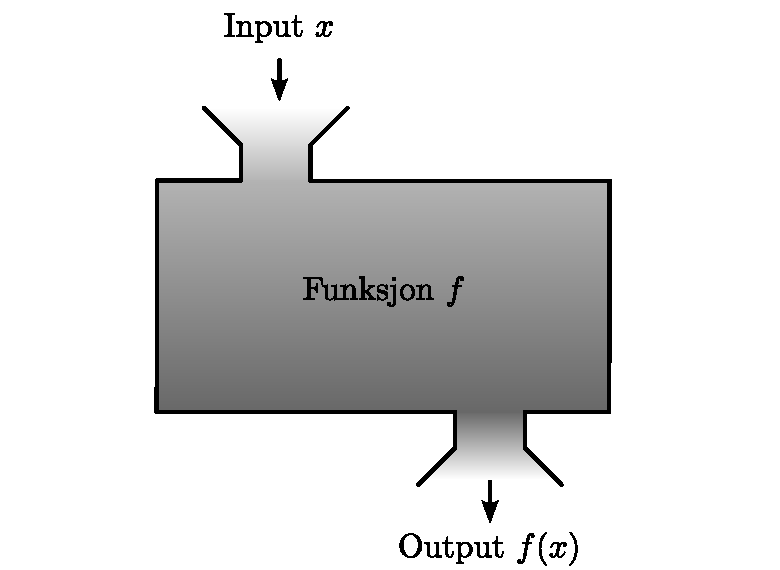
\includegraphics[width=0.8\textwidth]{function_blackbox}    
% \end{center}

% Hvis vi for eksempel ser på den matematiske funksjonen
% $$f(x) = x^2 + 3x + 1.$$
% Så kan vi for hver verdi av $x$ (input) beregne en resulterende verdi av $f(x)$ (output). Med andre ord er funksjonen $f$ en slags regel, eller maskin, som behandler et tall vi gir den. Vi kan definere denne funksjonen i Python som følger
% \begin{lstlisting}
% def f(x):
%     return x**2 + 3*x + 1    
% \end{lstlisting}
% \vspace{-0.3cm}
% her er \verb+def+ og \verb+return+ Python-kommandoer som vi skal forklare litt mer i detalj snart. Kort fortalt definerer vi her at det skal finnes en funksjon som heter $f$, som tar et tall $x$ inn, og gir tilbake (returnerer) tallet $f(x)$. Vi kan bruke funksjonen, vi kaller dette gjerne å "kalle på funksjonen", som følger
% \begin{lstlisting}
% print f(2)
% print f(3.5)
% print f(-1) + f(1)
% \end{lstlisting}
% \vspace{-0.3cm}
% som gir:
% \begin{lstlisting}
% 11
% 23.75
% 4
% \end{lstlisting}
% \vspace{-0.3cm}
% Så fort vi har definert en funksjon i python, huskes denne helt til programmet er ferdig å kjøre, og vi kan bruke den så mye vi ønsker. Funksjoner vi definerer, er egentlig bare en ny type variabel.

% En funksjon i python, trenger ikke nødvendigvis å være matematisk. Vi kan for-eksempel lage en funksjon som følger
% \begin{lstlisting}
% def greet(name):
%     print "Hello " + name + "!"
% \end{lstlisting}
% \vspace{-0.3cm}
% Denne funksjonen tar et navn som input, det vil si, en tekst-streng, og skriver ut en hilsen som output. Kommandoen
% \begin{lstlisting}
% greet("Lucy")
% \end{lstlisting}
% \vspace{-0.3cm}
% resulterer altså i
% \begin{lstlisting}
% Hello Lucy!
% \end{lstlisting}
% \vspace{-0.3cm}
% Merk at denne funksjonen ikke brukte kodenavnet \verb+return+, og når vi kallet på funksjonen, skrev vi ikke \verb+print+ før funksjonskallet. Dette er fordi funksjonen i seg selv printet, det var det vi hadde \emph{definert} at den skulle gjøre. Det er kanskje litt vanskelig å skjønne denne forskjellen, så la oss se på et par eksempler til.

% Vi definerer to funksjoner, $f_1$ og $f_2$. Vi vil at de begge skal ta et tall $x$ som input, og regne ut $2x$, altså det dobbelte. Forskjellen skal være at $f_1$ returnerer resultatet, mens $f_2$ printer det. Vi har altså:
% \begin{lstlisting}
% def f1(x):
%     return 2*x

% def f2(x):
%     print 2*x
% \end{lstlisting}
% \vspace{-0.3cm}
% La oss nå prøve å kalle på $f_1$ og $f_2$ på forskjellige måter og prøve å forstå hva som skjer. Først skriver vi:
% \begin{lstlisting}
% f1(2)
% \end{lstlisting}
% \vspace{-0.3cm}
% Vi får ikke noen feilmelding, så det virker greit. Men vi får heller ingen utskrift, det skjer ingenting! Dette er fordi vi kaller på $f_1$ med tallet 2 som input, funksjonen regner ut at $2*2 = 4$, og returnerer verdien, men så gjør vi ingenting med denne verdien. Vi kunne for eksempel gjort
% \begin{lstlisting}
% a = f1(2)
% print a
% \end{lstlisting}
% \vspace{-0.3cm}
% Her lagrer vi den returnerte verdien i en variabel \verb+a+, og så skriver vi ut \verb+a+. Nå får vi resultatet til skjerm, som er 4, flott!

% La oss nå prøve
% \begin{lstlisting}
% f2(3)
% \end{lstlisting}
% \vspace{-0.3cm}
% Dette fungerer veldig fint, vi får resultatet 6, rett til skjerm, flotte saker. Dette er fordi vi kaller på funksjonen $f_2$, som skriver tallet rett til skjermen. Om vi nå derimot prøver å lagre resultatet i en variabel
% \begin{lstlisting}
% a = f2(3)
% print a
% \end{lstlisting}
% \vspace{-0.3cm}
% får vi et litt mystisk resultat:
% \begin{lstlisting}
% 6
% None
% \end{lstlisting}
% \vspace{-0.3cm}
% For å skjønne hva som skjer her, så må vi først tolke kodelinjen \verb+a = f2(3)+, som vi lærte forrige uke, så betyr en slik linje at vi skal regne ut det som er på høyre-siden, og lagre det i variabelen \verb+a+. Vel, på høyre side kaller vi på $f_2$ med tallet $x=3$, $f_2$ gjør som vi har definert å skriver ut resultatet $2*x=6$ rett til skjerm. Etter det er $f_2$ ferdig, men den har ikke \emph{returnert} noen verdi, så når \verb+a+ settes lik resultatet på høyre-siden, så blir den ingenting, eller \verb+None+ som det heter i Python.

% Du har forhåpentligvis fått en viss idé om hva det nå betyr at en funksjon returnerer en verdi ved hjelp av \verb+return+-kommandoen. Ikke få panikk om du synes dette er ganske forvirrende, forståelse kommer med tid i programmering, så du skjønner det nok bedre etter du har fått prøvd deg litt frem!

% \subsection{Funksjoner av flere variabler}
% Når man først vet hvordan man lager funksjoner i python, er det superenkelt å lage funksjoner av flere variabler. Vi kan for eksempel lage følgende funksjon
% $$f(x,y) = 2x^2 + xy + 3,$$
% som følger
% \begin{lstlisting}
% def f(x,y):
%     return 2*x**2 + x*y + 3

% print f(3,4)
% \end{lstlisting}
% \vspace{-0.3cm}
% Tilsvarende kan vi lage funksjoner som ikke tar noen argumenter. Disse er kanskje mer nyttig i en programmeringssammenheng enn i en matematisk sammenheng. Vi kan foreksempel lage en funksjon
% \begin{lstlisting}
% def greet():
%     print "Hey there! I hope you have a great day!"
% \end{lstlisting}
% \vspace{-0.3cm}
% Merk at for å kalle på en slik funksjon, må vi fortsatt bruke parantesene, slik at et kall på \verb+greet+ skrives
% \begin{lstlisting}
% greet()
% \end{lstlisting}

% En ting det er verdt å merke seg er at mange av kommandoene vi har brukt i Python hitil, er funksjoner som er definert på akkurat den måten vi har lagt frem nå. For eksempel er \verb+range+ en funksjon, som vi kaller på når vi bruker. Når vi skriver; \verb+range(1,10,2)+ så gjør vi et funksjonskall med 3 inputtall.

% \clearpage

% \section{Arrays}

% Vi skal snart gå inn på plotting i Python, som vil si å lage figurer. Men da bør vi først nevne \verb+arrays+. Arrays er en spesiell type liste ment for matematikk. I motsetning til lister, som kan inneholde forskjellig type innhold, så kan arrays bare inneholde tall. Lister kan også gjøres større og mindre ved å legge til eller slette elementer, mens arrays \emph{alltid} har samme antall elementer. Om vi lager en array med tusen tall, så vil den arrayen alltid ha tusen tall, vi kan derimot endre hvilke tall den inneholder.

% Dere skal nå få se de to vanligste måtene å lage arrays på. Først, et tomt array. Ettersom at et array alltid har likt antall plasser, må vi spesifisere størrelsen på arrayet. Vi bruker kommandoen \verb+zeros+:
% \begin{lstlisting}
% x = zeros(3)    
% \end{lstlisting}
% \vspace{-0.3cm}
% Variabelen \verb+x+ er nå et array, med tre elementer. Der alle er satt til tallet 0. Dette virker kanskje litt rart å gjøre, men vi kan nå endre spesifikke elementer ved å indeksere på følgende måte
% \begin{lstlisting}
% x[0] = 10
% x[1] = 4
% x[2] = 3
% \end{lstlisting}
% \vspace{-0.3cm}
% Firkantparantesene kalles "indeksering", og brukes for å få tilgang til enkelt elementer av et array eller en liste. Python starter å telle på 0, så \verb+x[0]+ er det første elementet, og \verb+x[1]+ det andre, osv.
% Om vi nå skriver \verb+print x+ får vi nå resultatet
% \begin{lstlisting}
% [ 10.   4.   3.]
% \end{lstlisting}
% \vspace{-0.3cm}

% Neste måte lage et array på, er med funksjonen \verb+linspace+, som står for \emph{linear spacing}. Den tar tre inputparamtere: start, stop, antall.Om vi for eksempel skriver
% \begin{lstlisting}
% x = linspace(0,10,11)
% print x
% \end{lstlisting}
% \vspace{-0.3cm}
% får vi 
% \begin{lstlisting}
% [ 0.   0.2  0.4  0.6  0.8  1. ]
% \end{lstlisting}
% \vspace{-0.3cm}
% Altså er \verb+x+ et array med 6 elementer, hvor det første elementet er 0, det siste 1, og de resterende er jevnt fordelt. Vi kommer til å se at linspace er veldig praktisk når vi skal plotte.

% \subsection{Vektoriserte funksjoner}
% En stor fordel med arrays, er at de er laget for å drive med matematikk. Arrays oppfører seg foreksempel akkurat som vektorer. Det betyr at vi kan for eksempel bruke arrays til å regne prikkprodukt og kryssprodukt
% \begin{lstlisting}
% u = array([1,-4,3])
% v = array([3,2,-1])
% print dot(u,v)
% print cross(u,v)
% \end{lstlisting}
% \vspace{-0.3cm}
% \begin{lstlisting}
% -8
% [-2 10 14]
% \end{lstlisting}
% \vspace{-0.3cm}

% En annen veldig nyttig funksjonalitet, er at vi kan kalle på funksjoner med arrays som input, om vi for eksempel har laget funksjonen som vi så på tidligere
% \begin{lstlisting}
% def f(x):
%     return x**2 + 3*x + 1
% \end{lstlisting}
% \vspace{-0.3cm}
% så kan vi kalle på denne med et array som følger
% \begin{lstlisting}
% a = array([0,1,2,3,4,5])
% print f(a)
% \end{lstlisting}
% \vspace{-0.3cm}
% \begin{lstlisting}
% [ 1  5 11 19 29 41]
% \end{lstlisting}
% \vspace{-0.3cm}
% Det som skjer når vi kaller på funkjsonen med et array, er at Python regner ut resultatet element for element og returnerer et array med resultatene tilbake.

% \section{Plotting}
% Vi skal nå se på plotting i Python, som vil si å lage enkle figurer og grafer. Vi kommer til å tegne inn grafen vår i et koordinatsystem som vi er vant med fra matematikk. For å plotte bruker vi funksjonen \verb+plot+ fra pakken Pylab, som tar som input to lister, eller arrays, av tall. Vi kan altså for eksempel skrive
% \begin{lstlisting}
% plot([0,0.5,1], [2,4,6], 'x')
% show()
% \end{lstlisting}
% \vspace{-0.3cm}
% Her tegnes altså punktene (0,2), (0.5,4) og (1,6) inn i koordinatsystemet.
% Vi må bruke kommandoen \verb+show()+ for å vise figurer vi har laget. Vi har også lagt inn tekstrengen \verb+'x'+ i plotte-kommandoen, det er for at den skal tenge punktene vi gir som kryss. Hvis vi ikke ber den tegne kryss, tegner den rett og slett rette streker mellom punktene.

% Om vi har definert en funksjon, for eksempel:
% $$f(x) = x^2 + 3x + 1,$$
% som vi har sett på tidligere. Kan vi nå gjøre som følger
% \begin{lstlisting}
% def f(x):
%     return x**2 + 3*x + 1

% x = linspace(-6,6,1000)
% y = f(x)

% plot(x,y)
% show()
% \end{lstlisting}
% \vspace{-0.3cm}
% Her lager vi altså et sett med tusen punkter, som vi så plotter. Vi får dermed en fin figur av funksjonen $f(x)$. 

% Tilsvarende kan vi lage plot av velkjente matematiske funksjoner, for eksempel sinus og cosinus.
% \begin{lstlisting}
% x = linspace(0,2*pi,1000)
% plot(x,sin(x))
% plot(x,cos(x))
% show()
% \end{lstlisting}
% \vspace{-0.3cm}
% Merk at siden vi ga to plotte kommandoer før vi brukte show, så får vi to kurver i samme figur.

% Etter vi har lagd kurven ved å bruke \verb+plot+-kommandoen, og før vi bruker \verb+show+, så kan vi pynte på figuren vår. Vi kan for eksempel legge til navn på akser med
% \begin{lstlisting}
% xlabel('x')
% ylabel('y')
% \end{lstlisting}
% \vspace{-0.3cm}
% Vi kan lage tittel på figuren med \verb+title+-funksjonen på samme måte. Vi kan definere hvilke deler av figuren vi skal vise med \verb+axis+, for eksmepel
% \begin{lstlisting}
% axis([0,2*pi,-1,1])
% \end{lstlisting}
% \vspace{-0.3cm}
% vi gir altså en liste med \verb+[xstart, xstop, ystart, ystop]+.

% Vi kan også lagre figuren vår med
% \begin{lstlisting}
% savefig('figure1.png')
% savefig('figure1.pdf')
% \end{lstlisting}
% \vspace{-0.3cm}
% som lagrer bilde som filene 'figure1.png' og 'figure2.pdf' henholdsvis.

% Det er mange andre muligheter for å pynte på plot og få dem til å se kule ut, men la oss ikke dykke for dypt inn i det akkurat nå. Vi kommer til å se mer på plotte-muligheter iløpet av ukene som kommer, men om du er utålmodig kan du se på \url{matplotlib.org} som er nettsiden til plottepakken som pylab bruker, der finnes det mange eksempler på plots man kan lage.



% \clearpage


% \section*{Oppgave 1}
% \begin{itemize}
% \item[(a)] Definer en funksjon \verb+celsius_to_fahrenheit+ som tar grader $C$ som input, og returnerer grader Fahrenheit. Vi minner om at formelen for omregningen er
% $$F = \frac{9}{5}C + 32.$$
% \item[(b)] Bruk funksjonen til å finne ut hvor mange grader Fahrenheit disse tempraturene er: $20^\circ$, $0^\circ$, $-40^\circ$. 
% \item[(c)] Skriv en løkke der du lar gradier i Celsius gå fra -100 til 100 og skriv ut de tilhørende gradene i Fahrenheit ved å bruke funksjonen din. \\ \textbf{Hint 1:} Bruk \texttt{range}-funksjonen \\
% \textbf{Hint 2:} Du må kalle på funksjonen din inne i løkka.
% \end{itemize}


% \section*{Oppgave 2}
% Vi skal nå bruke løkker og \verb+range+-funksjonen til å regne ut noen matematiske summer
% \begin{itemize}
%     \item[(a)] Regn ut summen av alle oddetall under 1000.
%     \item[(b)] Regn ut summen av alle kvadrattall til og med 10000. \\ \textbf{Hint:} Vi er altså ute etter summen
%     $$1 + 4 + 9 + 16 + \ldots + 10000 = \sum_{i=1}^{100} i^2.$$
%     \item[(c)] Regn ut summen av den uendelige rekka
%     $$1 + \frac{1}{2} + \frac{1}{4} + \frac{1}{8} + \ldots$$
%     \textbf{Hint:} Hvert ledd i summen blir mindre og mindre, det holder altså å ta med for eksempel de 1000 første leddene. Da alle ledd etter dette vil bidra ekstremt lite til det endelige svaret
% \end{itemize}

% \section*{Oppgave 3}
% \begin{itemize}
%     \item[(a)] Plot $e^x$ for $x\in[0,2]$.
%     \item[(b)] Lag et plot, der du viser de tre funksjonene:
%     $$e^x, \qquad e^{-x}, \qquad 1/e^{x}.$$
%     for $x \in [0,2]$. Her må du bruke \verb+axis+-kommandoen for å velge rimelige akser på figuren din!
%     \item[(c)] Pynt på plottet du nettopp lagde ved hjelp av funksjonene \verb+axis+, \verb+xlabel+, \verb+legend+, \verb+title+ og \verb+grid+.
%     \item[(d)] Lagre plottet ditt som en .pdf-fil, og som en .png-fil. Sjekk at filene ble lagret riktig og at de ser ut som forventet.
% \end{itemize}



% \clearpage

% \section*{Utfordringer!}
% \subsection*{Primtall}
% Greier du å skrive en funksjon som tar et heltall som input, og finner ut om det er et primtall eller ikke?
% \subsection*{Fibonacci}
% Greier du å skrive et program som regner ut og skriver ut Fibonacci-tallene?
% \subsection*{Project Euler}
% På nettsiden \url{www.projecteuler.net} er det mange morsomme matematiske nøtter som er ment å løses ved programmering. Se om du greier å få til et par av de første oppgavene. Spør gjerne om hjelp.


% Denne uken kommer hovedsakelig til å gå med til repetisjon av tidligere programmering, for den delen er det greit å se på notatene fra forrige gang, samt å se på oppgavene vi har gitt dere der.

% Andre halvdel av denne uka kommer til å gå med til å starte å se på fysikken vi skal løse i de siste to ukene av prosjektet, og det er det vi skriver om i dette notatet.


% \section{Fallskjermhopping}

% Vi skal nå begynne å studere hvordan hastigheten til en person som hopper i fallskjerm endrer seg over tid. Vi kommer til å finne matematiske ligninger basert på vår fysiske forståelse av de kreftene som virker på hopperen. Vi skal diskutere ligningene vi kommer frem til, og se på hvorfor ikke greier å løse dem med kun penn og papir. Vi skal derfor se hvordan vi kan løse ligningene ved hjelp av programmering.


% Et fallskjermhopp består hovedsakelig av to deler. Den første delen er det som skjer før fallskjerm er utløst, denne delen kalles gjerne \emph{fritt fall}, i de fleste sportssammenhenger vil man oppleve ca ett minutt fritt fall per hopp. Etter dette utløser hopperen fallskjermen som da drastisk reduserer fallhastigheten, under fallskjerm brukeren hopperen så vanligvis fra ett til tre minutter videre ned til bakken avhengig av hvor stor fallskjerm de bruker og hvor nærme bakken de utløste skjermen.

% I begge faser utsettes hopperen bare for to krefer, tyngdekraft og luftmotstand. Så vi har
% $$\sum F = F_G + F_D,$$
% der $F_G$ er tyngdekraften og $F_D$ er luftmotstand. Dere har sikkert kjennskap til at tyngdekraften er gitt ved
% $F_G = mg,$
% der $m$ er den totale massen til hopperen, som vil se personvekten og alt utstyret, og $g$ er tyngdens akselersjonskonstant, som vi setter til $g=9.81$ m/s$^2$. En fallskjermhopper vil falle med veldig høy hastighet, og vi bruker derfor en kvadratisk form på luftmotstanden, som vi kan skrive som følger
% $$F_D = \frac{1}{2}\rho C A v^2,$$
% her er $\rho$ tettheten til luft, $C$ er luftmotstandskoeffisienten som avhenger av formen på objektet som faller og $A$ er frontarealet.
% For å slippe å skrive så mye kaller vi disse tallene samlet for $D$, slik at
% $$\frac{1}{2}\rho C A = D,$$
% $$F_D = -Dv^2.$$
% ligningen vi skal løse har altså følgende form
% $$ma = mg - D v^2.$$
% Dette er det som matematisk kalles en differensialligning, la oss diskutere hva det betyr.

% \section*{Differensialligninger}
% Tidligere når vi har sett på ligninger, så er det et matematisk uttrykk, der vi løser for en ukjent. For eksempel kan vi ha ligningen
% $$x^2 + 7 = 56.$$
% Dette er en ligning fordi vi har en "likhet". Og vi vet at vi kan løse denne for $x$, ved å flytt over konstanten $7$, og så ta roten, da finner vi at 
% $$x = \pm 7.$$
% Altså har vi løst ligningen, og funnet at $x$ er 7. En differnsialligning er også en ligning fordi den innholder en "likhet" på samme måte, og den har en ukjent vi løser for. Den store forskjellen er at den ukjente vi løser for, er ikke lenger et enkelt tall, men det er derimot en funksjon.

% Newtons 2.\ lov er et perfekt eksempel på en differensialligning, som vi løser for å finne enten farten, eller posisjonen, til et objekt. Her er både farten, og posisjonen, eksempler på funksjoner, fordi de endrer seg med tid: $v(t)$, $x(t)$. En differensialligning vil innholde den deriverte av funksjonen vi er ute etter, som er mer synlig om vi skriver akselerasjonen som den deriverte av hastigheten i Newtons 2.\ lov:
% $$\sum F = ma = m\frac{\d v}{\d t}.$$
% Differensialligningen vi prøver å løse er:
% $$m\frac{\d v}{\d t} = mg - D v(t)^2.$$

% Så, hvordan løser vi en slik ligning? Vel, det finnes utrolig mange forskjellige typer differensialligninger, og det finnes enda flere metoder før å løse dem! De som tar R2, kommer til å lære en del om å løse denne type ligninger, men vi har ikke tid til å dekke så altfor mye av det pensumet her.

% \subsection*{Uløslighet}
% Differensialligningen vi ønsker å løse er
% $$m\frac{\d v}{\d t} = mg - D v(t)^2,$$
% og vi ønsker å løse den for hastigheten $v(t)$. Men dette får vi ikke til, fordi akselerasjonen avhenger av hastigheten. Dette er nettopp grunnen til at vi ofte ser bortifra luftmotstand når vi løser Newtons 2.\ lov. Ofte er dette greit fordi resultatet er tilnærmet likt med og uten. Men, i visse tilfeller vil luftmotstand gi et veldig stort forskjell - og det er tilfellet i fallskjermhopping.

% \section{Fremgangsmåte}
% Så, hvordan kan vi løse en uløselig ligning ved hjelp av programmering? Idéen er ganske enkel, men la oss prøve å ta det steg for steg.

% La oss starte med å se på hvordan det hadde gått om vi hadde sett bortifra luftmotstand, da hadde vi hatt fritt fall
% $$ma = \sum F = mg,$$
% slik at akselerasjonen hadde vært konstant
% $$a = g.$$
% I det tilfellet hadde vi kunnet bruke bevegelsesligningene, som hadde gitt oss svarene
% $$v(t) = v_0 + at.$$
% og 
% $$x(t) = x_0 + v_0 t + \frac{1}{2}at^2.$$
% Altså ser vi at hastigheten vokser konstant for alltid. Som selvfølgelig ikke kan stemme, da vi vet at en fallskjermhopper vil treffe \emph{terminalhastighet} ganske fort.

% \subsubsection*{Terminalhastighet}
% Terminalhastigheten er den raskeste hastigheten et objekt kan falle med, og vi kan enkelt finne den uten å løse differensialligningene vår, vi vet at når luftmotstanden er like stor som tyngdekraften, så vil summen av kreftene på hopperen være 0, og da er akselerasjonen null og falleren faller med en konstant hastighet, nemlig terminalhastigheten. Vi har altså
% $$mg = \frac{1}{2}\rho C A v_T^2,$$
% når vi løser denne for terminalhastigheten har vi
% $$v_T = \sqrt{\frac{2mg}{\rho C A}},$$
% og når vi setter inn rimelige verdier ($m=90$ kg, $C=1.4$, $\rho=1$ kg/m$^3$, $A=0.7$ m$^2$, $g=9.81$ m/s$^2$) får vi
% $$v_T = 42.4 {\rm\ m/s} = 153 {\rm\ km/h}.$$

% \section{Bruke bevegelsesligningene med luftmotstand}
% Om vi nå legger til luftmotstanden igjen, vet vi at vi ikke kan bruke bevegelsesligningene, fordi vi ikke har konstant akselerasjon. Vi har
% $$a(v) = g - \frac{1}{2m}Dv^2,$$
% og ettersom at hastigheten øker, så vil akselerasjonen minke med tiden. Merk at vi skriver $a(v)$, fordi akselerasjonen er en funksjon av hastigheten. Om vi derimot ser på en veldig liten tidsendring $\Delta t$, så vet vi at hastigheten vil endre seg veldig lite, så vi kan bruke bevegelsesligningene et kort \emph{steg} frem i tid ved å si at akselerasjonen er konstant en kort tid:
% $$v_1 = v_0 + a(v_0)\Delta t.$$
% Nå har vi altså funnet hastigheten til hopperen en kort tid etter han startet. Vi kan nå gå enda litt lenger frem i tid, ved å oppdatere akselerasjonen, og si at den er konstant en ny kort tidsperiode
% $$v_2 = v_1 + a(v_1)\Delta t.$$
% Trikset her, er å la $\Delta t$ være veldig liten, slik at akselerasjonen er tilnærmet konstant. Vi må derfor ta veldig mange slike små tidsteg:
% $$v_{n+1} = v_n + a(t_n)\Delta t,$$
% og på denne måten kan vi løse differensialligningen vår et skritt av gangen til vi har funnet hele løsningen.

% \subsection{En mer matematisk tankemåte}
% Differensialligningen vår er
% $$a = g - \frac{D}{m}v^2,$$
% og vi kan skrive akselerasjonen som den deriverte av hastigheten
% $$\frac{\d v}{\d t} = g - \frac{D}{m}v^2.$$
% Definisjonen av den deriverte av $v$ er
% $$a = \frac{\d v}{\d t} = \lim_{\Delta t \to 0} \frac{v(t+\Delta t)-v(t)}{\Delta t}.$$
% Vi kan si at vi tilnærmer den deriverte ved istedenfor å la $\Delta t$ gå helt mot 0, at vi stopper den på et lite tall, vi har da at
% $$a = \frac{\d v}{\d t} \approx \frac{v(t+\Delta t) - v(t)}{\Delta t}.$$
% slik at
% $$v(t+\Delta t) = v(t) + a\Delta t.$$
% Vi ser altså at dersom vi kjenner farten ved tiden $t$, så kan vi finne den en kort tid senere ved å plusse på $a \Delta t$, der vi kan "late som" akselerasjonen er konstant.



% Vi er nå klare for å trekke sammen alle trådene vi har sett på så langt og begynne å lage et program som løser bevegelsesligningene for fallskjermhopping og strikkhopp. Vi starter med litt repetisjon av fysikken, og så ser vi på hvordan vi skal implementere det på datamaskin.


% \section*{Kreftene}


% Et fallskjermhopp består hovedsakelig av to deler. Den første delen er det som skjer før fallskjerm er utløst, denne delen kalles gjerne \emph{fritt fall}. Etter dette utløser hopperen fallskjermen som da drastisk reduserer fallhastigheten. I begge faser utsettes hopperen bare for to krefer, tyngdekraft og luftmotstand. Så vi har
% $$\sum F = F_G + F_D,$$
% der $F_G$ er tyngdekraften og $F_D$ er luftmotstand. Dere har sikkert kjennskap til at tyngdekraften er gitt ved
% $F_G = mg,$
% der $m$ er den totale massen til hopperen, som vil se personvekten og alt utstyret, og $g$ er tyngdens akselersjonskonstant.  En fallskjermhopper vil falle med veldig høy hastighet, og vi bruker derfor en kvadratisk form på luftmotstanden, som vi kan skrive som følger
% $$F_D = \frac{1}{2}\rho C A v^2,$$
% her er $\rho$ tettheten til luft, $C$ er luftmotstandskoeffisienten som avhenger av formen på objektet som faller og $A$ er frontarealet.

% Det eneste som endrer seg når fallskjerm løses ut, er frontarealet $A$, og luftmotstandskoeffisienten $C$. Ellers er fysikken helt lik.

% \subsection*{Parametere}
% Tallene $m$, $g$, $\rho$, $C$, $A$ er det som kalles fysiske parametere, og det er størrelser vi velger - vi velger dem utifra hva slags simulering vi ønsker å gjøre, men vi regner dem altså generelt sett som kjent. I vår simulering kan vi bruke følgende parametere
% \begin{center}
% \begin{tabular}{c|c}
% Fritt Fall \\ \hline
% $m$ & 90 kg \\ \hline
% $g$ & 9.81 m/s$^2$ \\ \hline
% $\rho$ & 1 kg/m$^3$\\ \hline
% $C$ & 1.4 \\ \hline
% $A$ & 0.7 m$^2$\\ \hline \hline
% Under fallskjerm \\ \hline
% $C_{\rm p}$ & 1.8 \\ \hline
% $A_{\rm p}$ & 44 m$^2$
% \end{tabular}
% \end{center}

% \subsection*{Newtons 2.\ lov}

% Om vi bruker Newtons 2.\ lov sammen våre kraftlover får vi et uttrykk fra akselerasjonen til fallskjermhopperen. Vi har:
% $$\sum F = ma,$$
% setter vi inn kreftene får vi
% $$F_g + F_d = ma,$$
% da har vi
% $$mg - \frac{1}{2}\rho C A v^2 = ma,$$
% vi deler på $m$ for å få et uttrykk for $a$:
% $$a = g - \frac{1}{2m}\rho C A v^2.$$
% Vi ser at akselerasjonen avhenger av hastigheten, så vi kan skrive den som en funksjon av $v$:
% $$a(v) = g - \frac{1}{2m}\rho C A v^2.$$

% \section*{Oppgave - Regne ut terminalhastigheten}
% Terminalhastigheten er den raskeste hastigheten et objekt kan falle med. Regn ut terminalhastigheten for fallskjermhopperen vi ser på. \\ 
% \textbf{Hint:} Ved terminalhastigheten faller man med konstant hastighet, da vet vi at akselerasjonen er null. Hva betyr dette med tanke på Newtons 2.\ lov?

% \clearpage

% \section*{Fremgangsmåte for å finne hastigheten til hopperen}
% Vi vet at dersom vi har en konstant akselerasjon, og en starthastighet $v_0$ så kan vi regne ut hastigheten ved en hvilken som helst tid $t$ utifra:
% $$v(t) = v_0 + at, \qquad \mbox{for konstant } a.$$
% Så hva gjør vi når vi \emph{ikke} har en konstant akselerasjon? I vårt tilfelle vil akselerasjonen endre seg over tid, fordi hastigheten endrer seg over tid. Men over en veldig kort tid $\Delta t$, så kan vi si at den er så godt som konstant, vi kan da si at
% $$v_1 = v_0 + a(v_0) \Delta t.$$
% Der $v_0$ er starthastigheten, $v_1$ er hastigheten etter ett \emph{tidssteg}, 
% altsa ved tiden $t_1 = \Delta t$.
% Vi skriver $a(t_0)$ for å tydliggjøre at vi bruker akselerasjonen som gjelder
%  ved starttiden. Siden vi nå kjenner $v_1$, så kan vi regne ut $a(v_1)$ fra uttrykket vårt for akselerasjonen, og bruke denne til å gå et tidssteg til:
% $$v_2 = v_1 + a(v_1) \Delta t.$$
% Og slik kan vi fortsette, vi kan alltid regne oss ett tidssteg frem, ved å bruke resultatet fra forrige tidssteg
% $$v_{n+1} = v_n + a(v_n)\Delta t,$$
% for $n=0,1,2,3,\ldots$.

% Slik fortsetter vi til vi har simulert nok tidssteg til å nå en slutttid vi har valgt på forhånd. Vi ønsker gjerne at $\Delta t$ skal være minst mulig, slik at vi får et mer nøyaktig resultat. For eksempel kan vi bruke $\Delta t = 0.01$ s i vår simulering, altså tar vi skritt på ett hundredelssekund frem i tid av gangen. I et vanlig fallskjermhopp er hopperen ca.\ 1 minutt i fritt fall, så vi lar sluttiden være $T=60$ sekunder. Det betyr at vi trenger å ta totalt
% $$n = \frac{T}{dt} = \frac{60 \mbox{ s}}{0.01 \mbox{ s}} = 6000,$$
% tidssteg.

% \clearpage 

% \section*{På tide å programmere}

% Vi er nå klare for å sette igang, her er malen på programmet dere kommer til å skrive:
% \begin{itemize}
%     \item[1] Importer pylab, det er alt vi kommer til å trenge.
%     \item[2] Skriv inn alle parameterene vi trenger, det vil si $m$, $g$, $\rho$, $A$, $C$, $A_{p}$, $C_{\rm p}$, $v_0$.
%     \item[3] Definer akselerasjonen som en funksjon av hastigheten. \\
%     \textbf{Hint:} \verb+def a(v):+, og husk å returnere noe!
%     \item[4] Definer $\Delta t = 0.01$ (Hint: kall variablen \verb+dt+ i programmet ditt), $T=60$ og $n = T/dt$
%     \item[5] Opprett to \emph{arrays}, ett for hastigheten $v$ og et for tiden $t$. Vi vil at de skal være tomme, og ha plass til $n+1$ elementer, så bruk \verb+zeros+ kommandoen. Merk at nå vil \verb+v[i]+ i programmet ditt svare til $v_i$ i matematikken.
%     \item[6] Lag en \verb+for+-løkke som går over $i=0,1,2,\ldots,n$. (Hint, bruk \verb+range+.)
%     \item[7] Inne i løkka, regn ut $v[i+1]$ fra $v[i]$ ved å bruke formelen vi har funnet. Oppdater også tiden (Hint: \verb!t[i+1] = t[i] + dt!).
%     \item[8] Plot resultatet for å sjekke at alt har blitt gjort riktig (Hint: \verb+plot(t,v)+).
% \end{itemize}

% \section*{Oppgaver}
% Etter at du har fått programmet ditt til å funke kan du besvare følgende oppgaver
% \begin{itemize}
%     \item[a)] Pynt på plottet ved å lagge til navn på aksene (\verb+xlabel+ og \verb+ylabel+), et grid (\verb+grid()+) og eventuelt tittel og lignende.
%     \item[b)] Hvor lang tid tar det før falleren har nådd tilnærmet terminalhastighet? Les av plottet.
%     \item[c)] Skriv ut terminalhastigheten hopperen får i programmet ditt. Hint: Det er en funksjon \verb+max+, som henter ut det største elementet i et array. Sammenlign denne med terminalhastigheten du fant med penn og papir tidligere, hvor like blir verdiene? Ser det ut som programmet ditt regner riktig?
% \end{itemize}

% \clearpage

% \section*{Videre}
% Nå har vi laget et program, som finner hastigheten til hopperen under fritt fall med luftmotstand. Men vi må fortsatt legge til at fallskjerm utløses. Vi kommer til å se på dette i fellesskap neste gang, men de av dere som har fått til alt så langt, kan begynne å bryne dere på hvordan vi skal gjøre dette. Grunnidéen er ihvertfall denne: det er bare frontarealet $A$ og luftmotstandskoeffisienten $C$ som endrer seg når fallskjerm løses ut, så hvis vi greier å endre disse verdiene i programmet vårt til riktig tidspunkt, så simulerer vi effektivt at fallskjerm er løst ut. I løkka vår, så har vi tiden $t_i$, så kanskje vi greier å bruke en \verb+if+-test til å endre $A$ og $C$ til riktig tid?

% Neste gang kommer vi også til å regne ut og plotte $g$-kreftene fallskjermhopperen opplever. Vi kommer også til å finne hastigheten til en strikkhopper på samme måte som vi har gjort for fallskjermhopperen idag.


% Sist uke laget vi et program som løste bevegelsesligningene for fallskjermhopping. Vi startet med Newtons 2.\ lov, og så på kreftene som virket. Fra dette fant vi et uttrykk for akselerasjonen, og vi brukte så bevegelsesligningene vi vent gjelder ved konstant akselerasjon til å løse for hastigheten små steg fremover i tid.

% Idag skal vi gjøre det samme for posisjon, og vi skal da se på strikkhopp som et eksempel. Når vi ser på strikkhopp, er det egentlig bare uttrykket for akselerasjon som endrer seg, alt annet kan være helt likt. Men ettersom at kreftene som virker på en strikkhopper avhenger av posisjonen til hopperen, må vi også løse for posisjonen.

% Etter vi har sett på det kommer vi til å plott $g$-kreftene både for fallskjerm- og strikkhopperen. Vi kan da sammenligne strikk og fallskjermhopp baser på $g$-kreftene hopperen føler. Vi kommer også til å se på hvordan fallskjermen løses ut, og hvordan det påvirker $g$-kreftene hopperen utsettes for.

% \clearpage

% \section*{Å løse for posisjon}
% Sist uke fant vi først et uttrykk for akselerasjonen for en fallskjermhopper som var
% $$a(v) = g - \frac{1}{2}C\rho A v^2.$$
% og vi brukte så bevegelsesligningene som gjelder ved konstant akselerasjon
% $$v = v_0 + a t,$$
% til å ta små "tidssteg" på $\Delta t$, som ga oss
% \begin{align*}
% v_1 &= v_0 + a(v_0)\Delta t \\  
% v_2 &= v_1 + a(v_1)\Delta t \\
% v_3 &= v_2 + a(v_2)\Delta t \\
% &\hdots \\
% v_{i+1} &= v_i + a(v_i)\Delta t.
% \end{align*}

% Vi har også en bevegelsesligning ved konstant akselerasjon som gjelder for posisjon
% $$x = x_0 + v_0 t + \frac{1}{2}at^2,$$
% vi kan bruke denne til å ta "tidssteg" på samme måte som for hastigheten
% \begin{align*}
% x_1 &= x_0  + v_0 \Delta t + \frac{1}{2} a(v_0) \Delta t^2 \\  
% x_2 &= x_1  + v_1 \Delta t + \frac{1}{2} a(v_1) \Delta t^2 \\  
% x_3 &= x_2  + v_2 \Delta t + \frac{1}{2} a(v_2) \Delta t^2 \\  
% &\hdots \\
% x_{i+1} &= x_i + v_i\Delta t + \frac{1}{2} a(v_i)\Delta t^2.
% \end{align*}

% \clearpage

% \section*{Strikkhopp}
% La oss nå se på en strikkhopper og kreftene som virker på henne. Vi kan tenke på strikken som en slags fjær når den er strukket ut. Men når strikken er "trykket" sammen gir den ingen kraft (i motsetning til en fjær, som virker "begge veier"). Når hopperen hopper fra toppen av en bru, er strikken slynget sammen, og kommer derfor ikke til å påvirke hopperen før hun har falt langt nok til at strikken begynner å bli strukket ut.  Vi kaller punktet der strikken akkurat ikke er begynnt å bli strukket ut for likevektspunktet.

% La oss nå lage et referansesystem som passer bra til problemet vi ser på. Vi plasserer $x=0$ i likevektspunktet. Vi sier at strikken er 20 meter lang, så hopperen hopper fra et punkt som er 20 meter høyere enn likevektspunktet, altså i $x_0 = 20$ m. La oss også si at det går en elv under brua, og at brua er 60 m over elva.

% \begin{figure}[h!b]
% \centering
% 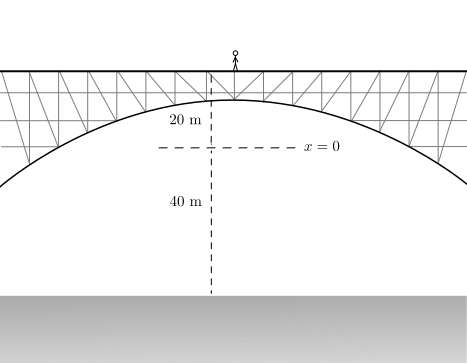
\includegraphics[width=0.9\textwidth]{Bungee_bridge}
% \end{figure}

% Vi ser nå at dersom posisjonen til hopperen er over likevektspunktet, så vil strikken ikke være strukket ut, og den virker ikke med noen kraft på hopperen. Siden vi har plassert likevektspunktet i $x=0$, betyr dette at strikkraften, som vi vil kalle $S$, er 0 hvis $x>0$.

% Hvis $x<0$ derimot, ser vi at strikken er strukket ut, og vil dermed trekke hopperen oppover med en fjærkraft. Denne fjærkraften modellerer vi med det som kalles Hooke's lov, som sier at kraften fra en fjær som er strukket ut en lengde $x$ er gitt ved:
% $$F = -kx,$$
% der $k$ er fjærstivheten. 

% Vi kan altså uttrykke den kraften fra strikken som en funksjon av posisjonen $x$ som følger:
% $$S(x) = \begin{cases} 0 & \mbox{hvis } x>0 \\
% -kx & \mbox{hvis } x \leq 0
% \end{cases}.$$

% I tilegg til snorkraften $S(x)$, virker det en tyngdekraft $mg$, og en luftmotstand $Dv$, på hopperen. Fra Newtons 2.\ lov
% $$\sum F = ma,$$
% har vi da
% $$S(x) - mg - Dv = ma.$$
% Vi løser for akselerasjonen, som vi nå ser er en funksjon av både posisjon og hastighet:
% $$a(x,v) = \frac{S(x)}{m} - g - \frac{D}{m}v.$$

% Ettersom at akselerasjon nå er en funksjon av både hastighet og posisjon, må vi løse for hastighet og posisjon samtidig, så vi har
% \begin{align*}
% v_1 &= v_0 + a(x_0, v_0)\Delta t \\
% x_1 &= x_0 + v_0\Delta t + \frac{1}{2}a(x_0, v_0)\Delta t^2 \\
% v_2 &= v_1 + a(x_1, v_1)\Delta t \\
% x_2 &= x_1 + v_1\Delta t + \frac{1}{2}a(x_1, v_1)\Delta t^2 \\
% &\hdots \\
% v_{i+1} &= v_i + a(x_i, v_i)\Delta t \\
% x_{i+1} &= x_i + v_i\Delta t + \frac{1}{2}a(x_i, v_i)\Delta t^2 \\
% \end{align*}

% \clearpage

% \section*{Kode strikkhopp}
% Du skal nå endre programmet du skrev sist uke til å løse for strikkhopping. Her er malen på hva programmet skal inneholde
% \begin{enumerate}
%     \item Importer pylab, det er alt vi kommer til å trenge.
%     \item Skriv inn alle parameterene vi trenger. Bruk $m=60$, $v_0=0$, $x_0=20$, $D=10$. Gjett på en verdi for fjærstivheten $k$, vi kommer til å justere den etterhvert.
%     \item Definer snorkraften $S(x)$. Her må du bruke \verb+def+ til å definere en funksjon, og en \verb+if+-test inne i funksjonen for å sjekke om $x>0$ eller $x<=0$. 
%     \item Definer akselerasjonen som funksjon av både posisjon og hastighet. \verb+def a(x,v):+.
%     \item Definer $\Delta t = 0.01$ (Hint: kall variablen \verb+dt+ i programmet ditt), $T=60$ og $n = T/dt$
%     \item Opprett tre \emph{arrays}, ett for hastigheten $v$, ett for posisjonen $x$ og ett for tiden $t$. Vi vil at de skal være tomme, og ha plass til $n+1$ elementer, så bruk \verb+zeros+ kommandoen. 
%     \item Sett første element i $x$-arrayet til å være $x_0$. Altså \verb+x[0] = x0+.
%     \item Lag en \verb+for+-løkke som går over $i=0,1,2,\ldots,n$. (Hint, bruk \verb+range+.)
%     \item Inne i løkka, regn ut $t[i+1]$, $v[i+1]$ og $x[i+1]$. Fra de følgende formlene
%     \begin{align*}
%     t_{i+1} &= t_i + \Delta t, \\
%     v_{i+1} &= v_i + a(x_i, v_i)\Delta t, \\
%     x_{i+1} &= x_i + v_i\Delta t + \frac{1}{2}a(x_i, v_i)\Delta t^2.
%     \end{align*}
%     Vi har altså
%     \begin{lstlisting}
% for i in range(n):
%     t[i+1] = t[i] + ...
%     v[i+1] = v[i] + ...
%     x[i+1] = x[i] + ...    
%     \end{lstlisting}
%     \item Plot resultatet for å sjekke at alt har blitt gjort riktig (Hint: \verb+plot(t,x)+).
% \end{enumerate}

% \subsection*{Oppgave}
% \begin{itemize}
%     \item[a)] Pynt på plottet ditt. Sett navn på akser osv.
%     \item[b)] Ved å se på plottet, prøv å juster fjærstivheten $k$ sånn at hopperen akkurat rører vannet. Altså at bunnen av kurven akkurat når $-40.$
%     \item[c)] Skriv ut makshastigheten hopperen opplever. Hint: \verb+max(v)+. Hvordan er dette sammenlignet med makshastigheten til fallskjermhopperen?
% \end{itemize}

% \clearpage

% \section*{Plotte $g$-krefter}
% Begrepet $g$-kraft er noe misvisende, da det egentlig ikke er snakk om "krefter" man opplever - men akselerasjon. Når menneskekroppen blir akselerert, føler vi dette som vekt. Tenkt for eksempel når du sitter i en bil som kjører gjennom en sving, og du blir "dratt" til siden. Disse akselerasjonene føles altså ut som en slags kraft på kroppen, og det er derfor vi snakket om $g$-krefter. Bokstaven "g" i $g$-kraft står for gravitasjon, og det er fordi vi sammenligner den kraften en person med tyngdekraften. Når du står helt i ro, føler du $1g$ fra tyngdekraften. I en berg-og-dalbane vil man etterhvert som man følger banen oppleve mye forskjellige $g$-krefter etterhvert som man akselerer inn og ut av svinger og opp og ned bakker. Når vi har et hurtig dykk nedover på en berg-og-dalbane blir man vektløs, som altså er $0g$, eller fritt fall. En fordel med å snakke om $g$-krefter fremfor de faktiske fysiske kreftene som virker på et objekt, er at de ikke avhenger av massen. Alle personer vil altså kjenne de samme $g$-kreftene i den samme berg-og-dalbanen.

% For å regne ut $g$-kreftene hopperen føler i begge tilfeller trenger vi egentlig bare å legge til et nytt array i løkka, hvor vi regner ut akselerasjonen som virker på hopperen, deler på $g$ og legger til 1. Koden er som følger:
% \begin{lstlisting}
% gforces = zeros(N+1)
% ...


% for i in range(N):
%     t[i+1] = t[i] + ...
%     v[i+1] = v[i] + ...
%     x[i+1] = x[i] + ...
%     gforces[i] = a(x[i],v[i])/g + 1
% \end{lstlisting}

% \subsection*{Oppgave}
% Regn ut og plot $g$-kreftene som virker på både fallskjerm- og strikkhopperen i programmet ditt. Sammenlign plottene, er de forskjellige? Forklar så godt du kan hvorfor de to er forskjellige.

% \clearpage

% \section*{Utløse fallskjermen}
% Vi har nå kommet til tidspunktet der vi skal løse ut fallskjermen i programmet vårt. Vi har nevnt tidligere at det eneste vi egentlig trenger å gjøre er å endre luftmotstandskoeffisienten $C$ til $C_{\rm P} = 1.8$ og frontarealet $A$ til $A_{\rm p} = 44$. Vi har hitill simulert fallskjerm hopperen i $T=60$ sekunder, la oss øke denne tiden til 180 sekunder. Men vi lar fortsatt den første løkka bare gå over de første 60 sekundene, deretter endrer vi $C$ og $A$, og løser for de siste 120 sekundene, altså
% \begin{lstlisting}
% dt = 0.01
% T = 180
% n = int(T/dt)

% # Simuler de forste 60 sekundene
% for i in range(0, 60/dt):
%     t[i+1] = t[i] + dt
%     v[i+1] = v[i] + a(v[i])*dt
%     gforces[i] = 1 - a(v[i])/g

% # Endre C og A
% C = C_p
% A = A_p

% # Simuler de siste 120 sekundene
% for i in range(60/dt, 180/dt):
%     t[i+1] = t[i] + dt
%     v[i+1] = v[i] + a(v[i])*dt
%     gforces[i] = 1 - a(v[i])/g
% \end{lstlisting}

% Nå kan vi plotte både hastigheten mot tid, og $g$-kreftene. Hva ser vi da? Et problem vi har fått er at vi endrer verdiene av $C$ og $A$ altfor brått. Dette er altså som om fallskjermen hadde blitt utløst umiddelbart, som hadde bremset ned hopperen enorm fort, og fører til nesten 100 $g$! Alt over 10 $g$ kan være livsfarlig og de fleste vanlige personer begynner å besvime når man går over $5$g.

% Moderne fallskjermer er defor laget for å løse seg ut saktere med vilje, det gir dermed en roligere nedbremsning. La oss prøve å simulere at fallskjermen bruker 5 sekunder på å løse seg fullstendig ut, og se hvordan de påvirker $g$-kreftene. Vi lager nå tre løkker. En helt uten skjerm, en der fallskjermen er i prosessen å løse seg ut, og en der skjermen er helt løst ut.

% \begin{lstlisting}
% dt = 0.01
% T = 180
% n = int(T/dt)

% # Simuler de forste 60 sekundene
% for i in range(0, 60/dt):
%     t[i+1] = t[i] + dt
%     v[i+1] = v[i] + a(v[i])*dt
%     gforces[i] = 1 - a(v[i])/g

% # Simulerer de neste 5 sekundene
% for i in range(60/dt, 65/dt):
%     C += (C_p-C)/(5/dt)
%     A += (A_p-A)/(5/dt)

%     t[i+1] = t[i] + dt
%     v[i+1] = v[i] + a(v[i])*dt
%     gforces[i] = 1 - a(v[i])/g

% # Simuler de siste 115 sekundene
% for i in range(65/dt, 180/dt):
%     t[i+1] = t[i] + dt
%     v[i+1] = v[i] + a(v[i])*dt
%     gforces[i] = 1 - a(v[i])/g
% \end{lstlisting}



\end{document}


“Programs must be written for people to read, and only incidentally for machines to execute.” 

